% ======================================================================
% TRB Annual Meeting Paper (unofficial template)
%
% A Differentiable Simulation Testbed for Longitudinal Train
% Dynamics: Reference Simulator, Real-Terrain Route Pipeline, and
% Research Console
%
% This paper reports the preliminary/infrastructure phase of an ongoing
% thesis. The learned surrogate itself is not trained or evaluated here.
%
% Build:  latexmk ltd_surrogate_trb.tex -pdf
% ======================================================================

\documentclass[numbered]{trbunofficial}

\usepackage{booktabs}
\usepackage{amssymb}

% Float placement: allow figures to share pages with text rather than
% being pushed onto pages of their own.
\renewcommand{\topfraction}{0.92}
\renewcommand{\bottomfraction}{0.85}
\renewcommand{\textfraction}{0.07}
\renewcommand{\floatpagefraction}{0.80}
\setcounter{topnumber}{2}
\setcounter{totalnumber}{3}

\begin{document}

% ---------- Title Page ----------
% Place Title Page AFTER \begin{document} and BEFORE \maketitle
% to include the front matter in page count

\title{A Differentiable Simulation Testbed for Longitudinal Train Dynamics: Reference Simulator, Real-Terrain Route Pipeline, and Research Console for a Graph Neural Surrogate}

% \TRBauthor[*]{Name}{Affiliation}{Email}[Address][ORCID]
% NOTE: author order to be confirmed with Dr. Duong before submission.
\TRBauthor*{George James}{School of Engineering, Colorado State University Pueblo}{gl.james1@pack.csupueblo.edu}[2200 Bonforte Blvd., Pueblo, CO 81001]
\TRBauthor{Trung Duong, Ph.D.}{School of Engineering, Colorado State University Pueblo}{trung.duong@csupueblo.edu}[2200 Bonforte Blvd., Pueblo, CO 81001]
\TRBauthor{Md Islam, Ph.D.}{School of Engineering, Colorado State University Pueblo}{md.islam@csupueblo.edu}[2200 Bonforte Blvd., Pueblo, CO 81001]
\TRBauthor{Saqib Gulzar, Ph.D.}{School of Engineering, Colorado State University Pueblo}{saqib.gulzar@csupueblo.edu}[2200 Bonforte Blvd., Pueblo, CO 81001]

\AuthorHeaders{James, Duong, Islam, and Gulzar}

\maketitle

% ======================================================================
% ABSTRACT (structured, per TRB 2027 requirements)
% ======================================================================
\section{Abstract}

High-fidelity simulation of longitudinal train dynamics (LTD) resolves nonlinear slack couplers, per-vehicle grade and curvature, actuator lag, and power-limited traction, but its computational cost places it beyond the repeated evaluation required for data-driven control design and operational planning. A fast, differentiable surrogate would remove this barrier; training one, however, first requires a resource that does not yet exist in the open, namely a reproducible, real-terrain LTD data generator spanning a wide family of consists and corridors. This paper documents that testbed. The coupled-vehicle system is formulated as a chain graph whose tensorized node and edge state admits arbitrary consist length without padding, and the target surrogate is expressed as a physics-residual correction to a known force-balance right-hand side so that it remains differentiable end to end. Three components are documented against this formulation: a stage-verified reference simulator, a pipeline that converts OpenStreetMap track geometry and USGS elevation data into the fields the simulator consumes, and TrainSet, a desktop console that renders consists, routes, and control profiles as named, serializable artifacts shared by interactive and batch use.

\vspace{0.25\baselineskip}
\noindent\textbf{Objectives:}~Small inefficiencies in freight driving strategy compound into substantial fuel losses over a corridor, and improved control requires a system model. Freight dynamics are strongly nonlinear and vary with both consist composition and route profile, yet no public dataset spans that variation. Data-driven system identification is therefore required, which in turn requires a simulation environment able to generate dynamics across a family of consists and real routes. The objective of this work is to build that environment.

\vspace{0.25\baselineskip}
\noindent\textbf{Methods:}~Classical multi-body LTD is recast into a node/edge tensor representation in which vehicles are graph nodes, couplers are graph edges, and the learned component is a residual on a known physics right-hand side. A reference simulator is implemented in Python in eight verified stages, from a single powered vehicle through nonlinear slack couplers, $N$-vehicle assemblies, per-vehicle route sampling, and first-order actuator lag with power-limited traction. Route profiles are derived from OpenStreetMap geometry, resampled onto a uniform 10~m arc-length grid, fused with USGS 3DEP elevation, and differentiated with a Savitzky-Golay filter to yield grade and curvature.

\vspace{0.25\baselineskip}
\noindent\textbf{Findings:}~Stage-by-stage verification confirms that the simulator reproduces the phenomena distinguishing LTD from point-mass modeling: the deadband and sharp re-engagement of a slack coupler, monotonic head-to-tail decay of steady draft force under head-end power, coupler cycling driven by vehicles occupying different grades simultaneously, and divergence between commanded and achieved traction under a power ceiling. On a representative 49~km corridor the pipeline recovers a sustained climb near one percent from elevation data carrying meter-scale error, and consists of 126 to 133 vehicles run end to end under randomized driving commands.

\vspace{0.25\baselineskip}
\noindent\textbf{Novelty:}~The work contributes an openly documented, reproducible LTD data-generation testbed built on real corridor terrain, together with a graph-tensor formulation that makes consist length a property of the data rather than a fixed architectural dimension, which is the precondition for a train-agnostic dynamical surrogate.

\vspace{0.25\baselineskip}
\noindent\textbf{Practical Applications:}~The testbed supports energy-aware evaluation of driving strategy and coupler-force safety screening across consist makeups and corridors without proprietary tools, and holding out whole corridors provides direct evidence of whether a learned model transfers.

\newpage

% ======================================================================
\section{Introduction}\label{sec:intro}
% ======================================================================

Longitudinal train dynamics (LTD) concerns the motion and internal force distribution along the length of a train. A freight consist is a distributed mechanical system of tens to hundreds of coupled masses whose interactions with one another and with the track profile are strongly nonlinear \citep{Cole2006HandbookLTD}. Simulating those interactions faithfully requires solving differential equations for every vehicle in the chain, and the computational burden grows steeply with model fidelity, from reduced point-mass representations to full multibody dynamics \citep{Wu2016OverviewLTD}. At the high-fidelity end the cost is severe enough that whole-trip design optimization was, before parallelization, effectively intractable, requiring months of sequential computation \citep{wu2019highfidelity}.

This computational cost is the central obstacle, since control design and operational planning require the model to be evaluated hundreds or thousands of times within an optimization loop. A surrogate model addresses this by learning an approximate input-to-response mapping that evaluates in milliseconds while retaining the underlying physical structure. Surrogates complement rather than replace deterministic physics models: the simulator supplies the training data and physical grounding, and the surrogate supplies the speed.

The broader project to which this paper belongs targets a specific surrogate, namely a differentiable model of LTD that serves as the world model within a fuel-optimal control routine. Two properties govern the design. First, the model must accommodate consists of arbitrary length, because a surrogate restricted to the train lengths on which it was trained is of limited operational value. Second, it must be differentiable with respect to the control plan, because the objective is not to forecast a single run but to determine how the outcome shifts when traction and braking commands are adjusted.

Before any of this can be attempted, a more elementary problem must be addressed. Training a surrogate that generalizes across consists and corridors requires a dataset spanning that variation, and no such public dataset exists. Established LTD simulators are largely proprietary, in-house, or consortium-restricted (Table~\ref{tab:ltd_tools}), and none is packaged to emit thousands of labeled trajectories across randomized consists and real corridors. The prerequisite is therefore an environment capable of generating that data, with route profiles drawn from real track, since a surrogate trained on invented grade profiles would be a weak foundation for any subsequent claim about generalization to real corridors.

This paper documents that environment, reporting the completed preliminary phase of the project and deliberately stopping short of the learned model: no surrogate is trained, and no accuracy or speedup results are claimed.

% ======================================================================
\section{Objectives}\label{sec:objectives}
% ======================================================================

This paper pursues four objectives, each corresponding to a completed component of the testbed.

\begin{enumerate}
  \item To formulate the LTD prediction and control problem as a graph-tensor system in which vehicles are nodes, couplers are edges, and consist length is a property of the data rather than a fixed architectural dimension, and to state the learning target as a physics residual that keeps the model differentiable end to end (\customref{PROBLEM FORMULATION}{sec:problem}).
  \item To construct a reference LTD simulator in verifiable stages, from a single powered vehicle to an $N$-vehicle consist with nonlinear slack couplers, per-vehicle route sampling, actuator lag, and power-limited traction, with the boundary of its fidelity stated explicitly (\customref{REFERENCE SIMULATOR}{sec:refsim}).
  \item To develop an end-to-end pipeline that converts raw OpenStreetMap track geometry and USGS 3DEP elevation into the grade, curvature, and speed-limit arrays the simulator consumes, including corridor recovery as a graph problem, uniform arc-length resampling, and Savitzky-Golay smoothing and differentiation (\customref{ROUTE ACQUISITION}{sec:routes}).
  \item To provide TrainSet, a desktop research console that renders car types, trains, control profiles, and routes as named, serializable artifacts shared between interactive exploration and headless batch generation (\customref{TRAINSET}{sec:trainset}).
\end{enumerate}

The remainder of the paper reviews related work, states the problem formulation, and then documents each built component in turn before summarizing status and future work.

% ======================================================================
\section{Related Work}\label{sec:related}
% ======================================================================

\subsection{Classical Longitudinal Train Dynamics}

Classical LTD studies the motion of rolling stock along the longitudinal axis of the track, accounting for both whole-train motion and the individual motion of each vehicle \citep{Cole2006HandbookLTD}. LTD models form a ladder of fidelity, ranging from a single point mass, through a multi-mass system in which each vehicle is a rigid body with one longitudinal degree of freedom connected by nonlinear couplers and draft gears, to models with additional degrees of freedom that expose curving effects, in-train instabilities, and derailment. Each rung trades speed for fidelity \citep{Wu2016OverviewLTD}; the work reported here sits deliberately on the middle rung.

The standard computational scheme treats LTD as the repeated evaluation of all force elements, namely propulsion and curving resistance, grade, traction, dynamic and air brake, and coupler forces, followed by state propagation through a numerical solver \citep{Wu2018ComputingSchemesLTD}. This modularity is what makes surrogate substitution feasible, since a single module can be replaced by a learned component without disturbing the rest.

The principal difficulty lies in the vehicle connection system. Friction draft gears exhibit extreme nonlinearity, including hysteresis and stick-slip, that is difficult to both model and numerically solve \citep{Wu2016OverviewLTD}. These force-element computations are independent across couplers and therefore parallelizable, which \citet{Wu2018ComputingSchemesLTD} exploit through sequential, parallel, and hybrid computing schemes. The concentration of cost in a structurally local computation is precisely what motivates a graph-based residual surrogate, because the expensive part of the model is an edge quantity.

Benchmarking has historically been weak in this field. \citet{Spiryagin2017BenchmarkQuestions} introduced an international initiative defining shared input scenarios, operating conditions, and required outputs, motivated by the observation that most LTD tools evolved independently as in-house software with limited transparency into their numerical methods and assumptions. Table~\ref{tab:ltd_tools} summarizes representative tools. The pattern is consistent: capable simulators exist, but few are openly available, and none is packaged as a bulk data generator.

\begin{table}[!ht]
  \caption{Representative Longitudinal Train Dynamics Simulation Tools}\label{tab:ltd_tools}
  \begin{center}
  \small
  \begin{tabular}{@{}p{2.1cm}p{3.3cm}p{5.2cm}p{2.6cm}@{}}
    \hline
    Tool & Origin & Scope & Availability \\
    \hline
    TrainDy \citep{Cantone2008TrainDy} & UIC-oriented consortium & Freight LTD for operations and safety analysis & Specialized / consortium \\
    TOES & Developed for AAR-member railroads \citep{WheelRail2018TOES} & Comprehensive train dynamics for operating scenarios & Commercial / licensed \\
    TEDS \citep{FRA2019TEDSProject} & U.S. FRA-sponsored & Safety and risk evaluation, incident investigation, operations LTD & Publicly documented \\
    UM Train \citep{UMTrainPlugin} & Universal Mechanism suite & LTD within a multibody ecosystem & Commercial \\
    TDEAS \citep{Wei2014TDEAS} & Research and industry, China & LTD with energy analysis & Research / institutional \\
    CRE-LTS \citep{Spiryagin2017BenchmarkQuestions} & Centre for Railway Engineering, CQU & Benchmarking-ready research LTD simulator & Research / in-house \\
    \hline
  \end{tabular}
  \end{center}
\end{table}

\subsection{Data-Driven and Hybrid Modeling in Rail}

Data-driven rail modeling falls into three overlapping categories. The first embeds learned components within classical multibody or finite-element frameworks, substituting nonlinear mechanical behavior with surrogates at significant runtime reduction \citep{nie_data_driven_dynamics} or packaging a machine-learning replacement for a full multibody model through a standardized co-simulation interface, with substantial reductions in computation time \citep{zhou_surrogate_integration}. The second targets in-train forces, which are difficult to measure directly in service: supervised approaches map telemetry to coupler force estimates using causally structured convolutional networks \citep{zhang_in_train_forces}, with extensions adding transfer learning to generalize across couplers and configurations \citep{intrainnet}. The third operates above the dynamics entirely, approximating the evaluation of candidate schedules within an optimization loop \citep{liu_rescheduling_surrogate}.

Three limitations recur and shape the present study. First, generalization across consist configurations remains difficult: force-estimation models are often trained on narrow scenario subsets, and even with transfer learning, performance degrades where strong nonlinear vehicle-to-vehicle interaction dominates \citep{zhang_in_train_forces,intrainnet}. Second, reliance on simulated labels means simulator-to-reality discrepancy compounds through a purely data-driven mapping. Third, hybrid approaches that retain physical structure generally aim to replicate nominal simulator output rather than robustness under distribution shift. In nearly every case, the training data is generated by a tool the authors do not describe in reproducible detail, which is the specific gap this paper addresses.

\subsection{Learned Simulators, Graph Networks, and Sequence Surrogates}

The formulation adopted here draws on work that treats physical simulation itself as a learning target with explicit relational structure. \citet{sanchez2020gns} demonstrate that message-passing graph networks learn particle-based physics and generalize to system sizes unseen during training. The relevance to LTD is direct, since a consist is already a graph, and one built on that structure inherits the property responsible for that generalization, namely that the computation is local and shared rather than indexed to a fixed number of entities. Neural ordinary differential equations \citep{chen2018neuralode} supply the complementary mechanism, allowing a learned residual on a physics right-hand side to be integrated while remaining differentiable with respect to its inputs, the key property required by the downstream control application.

Sequence and operator models offer an alternative. Transformers replace recurrence with multi-head self-attention \citep{vaswani2017attention}, and neural operators learn a solution map rather than a single-step update; both have been applied to long-horizon forecasting and to PDE-governed dynamics. These are capable tools, but they are a poorer structural fit for the present problem. A sequence model must commit to a token layout, so a consist of varying length requires padding and masking, and generalization to an unseen length is an extrapolation the architecture does not naturally support. A graph defined over vehicles and couplers obtains this property intrinsically. The project accordingly treats the graph network as the primary architecture and a transformer variant as an ablation against which the structural claim is tested.

\subsection{Uncertainty as a Safety Margin}

Not every simulator input is known exactly: vehicle masses, resistance coefficients, coupler stiffness, route shape, and command execution all carry uncertainty, and a substantial literature addresses this through quantile regression \citep{koenker1978regression} and distribution-free coverage via conformal methods \citep{romano2019conformalized}. The present project uses that machinery narrowly. Because the surrogate is intended for fuel-optimal control rather than general-purpose forecasting, uncertainty enters primarily as a margin the controller must respect, namely keeping estimated coupler force below its limit with high probability, so the pinball loss is applied only to safety-relevant quantities, chiefly coupler force. This scope explains why the infrastructure documented below emits deterministic trajectories: parameter uncertainty is introduced by resampling the generator, not by making the simulator itself stochastic.

% ======================================================================
\section{Problem Formulation}\label{sec:problem}
% ======================================================================

The physics presented below is standard; what matters is how it is organized, because the simulator's outputs, the surrogate's training targets, and the surrogate's internal state all share a single layout regardless of the number of vehicles in the train.

\subsection{Classical Formulation}

Represent the train as a chain of $N$ vehicles indexed $i = 0,\ldots,N-1$ from lead to tail, connected by $N-1$ couplers. Let $x_i(t)$ and $v_i(t) = \dot{x}_i$ denote the longitudinal position and velocity of vehicle $i$ along the route, and let $m_i$ denote its mass. Between vehicles $i$ and $i+1$, coupler $i$ has extension $\delta_i$ (relative displacement from nominal spacing, positive in draft) and transmits force $F_i$ to the trailing vehicle. Collecting the external and control contributions on vehicle $i$ into $F_{\mathrm{ext},i}(t)$,
\begin{align}
  & \dot{x}_i = v_i, \\
  & m_i \dot{v}_i = F_{\mathrm{ext},i}(t) + F_{i-1}(t) - F_i(t),
  \label{eq:classical}
\end{align}
with $F_{-1} = F_{N-1} = 0$ when end forces are absent. Coupler forces follow constitutive laws $F_i = \phi_i(\delta_i, \dot{\delta}_i,\ldots)$, in which slack, asymmetric buff and draft stiffness, and damping enter; actuator lag and power limits introduce further per-vehicle states.

\subsection{Tensorized State Representation}

For learning, and for software that must accommodate variable train length, the same physics is organized into two arrays that make the vehicle-coupler graph explicit. A node tensor $\mathbf{H}(t) \in \mathbb{R}^{N \times d_n}$ collects $d_n$ channels per vehicle: position, velocity, internal actuator states where those are dynamic, and static attributes replicated per row (mass, Davis coefficients, traction capability, and force limits). An edge tensor $\mathbf{E}(t) \in \mathbb{R}^{(N-1) \times d_e}$ holds $d_e$ channels per coupler: extension $\delta_i$, relative speed $\dot{\delta}_i$, coupler force $F_i$, nominal spacing, slack half-width, and buff and draft stiffness and damping parameters. Over a discrete time grid, trajectories are stored as rollout tensors $\mathbf{X} \in \mathbb{R}^{T \times N \times d_n}$ and $\mathbf{E}_{\mathrm{hist}} \in \mathbb{R}^{T \times (N-1) \times d_e}$.

This layout keeps the structure of the physical problem visible, since each coupler row depends only on the two adjacent vehicle rows, mirroring the chain structure of Equation~\ref{eq:classical}. For this reason the train is treated as a graph rather than as a fixed-length sequence. A graph-based model processes trains of any length directly, passing information between neighboring vehicles one coupler at a time, with no padding or masking. Handling variable length as a consequence of the representation rather than as an engineering workaround is what makes the train-agnostic objective attainable.

\subsection{Dynamics and the Learning Target}

Let $\mathbf{H}_{\mathrm{dyn}}(t)$ denote the dynamic channels of $\mathbf{H}(t)$ and let $\mathbf{p}$ denote the fixed parameters. The differential part of the evolution is
\begin{equation}
  \frac{\mathrm{d}}{\mathrm{d}t}\,\mathrm{vec}\!\left(\mathbf{H}_{\mathrm{dyn}}(t)\right) = \mathcal{F}_n\bigl(\mathbf{H}(t), \mathbf{E}(t), \mathcal{U}(t), \mathcal{R}; t\bigr),
  \label{eq:node_evolution}
\end{equation}
where $\mathrm{vec}(\cdot)$ stacks the columns of its matrix argument into a single column vector, $\mathcal{U}$ denotes the control inputs, $\mathcal{R}$ the route profile, and $\mathcal{F}_n$ the assembled right-hand side obtained from Equation~\ref{eq:classical} together with the actuator relations. In the reference integrator, several edge channels, including $\delta_i$, $\dot{\delta}_i$, and $F_i$, are reconstructed algebraically at each evaluation from vehicle positions and velocities rather than integrated as separate states, so that
\begin{equation}
  \mathbf{E}(t) = \mathcal{G}_e\bigl(\mathbf{H}(t), \mathbf{p}\bigr)
  \label{eq:edge_map}
\end{equation}
for those channels, while Equation~\ref{eq:node_evolution} carries the true differential degrees of freedom. Here $\mathcal{G}_e$ denotes the algebraic reconstruction map defined by the coupler kinematics and constitutive laws, for example $\delta_i = (x_i - x_{i+1}) - L_{0,i}$ together with the associated force law. Were internal draft-gear states introduced in later work, Equation~\ref{eq:edge_map} would be supplemented by differential equations on the corresponding rows.

The surrogate does not learn $\mathcal{F}_n$ from a blank slate. It begins from the known physics right-hand side and learns a correction, so that the predicted rate of change takes the form $\mathcal{F}_n + \Delta\mathcal{F}_\theta$, where $\Delta\mathcal{F}_\theta$ is a message-passing graph network operating on $(\mathbf{H}, \mathbf{E})$ and the whole is integrated as a neural ODE \citep{chen2018neuralode}. Building physics into the model structurally, rather than supplying it as an input feature or as a soft penalty in the loss, anchors the surrogate's behavior for consists and routes it has not encountered.

\subsection{Inputs, Outputs, and Objective}

Every scenario is specified by a triple $(\mathcal{R}, \mathcal{C}, \mathcal{U})$: a route profile $\mathcal{R}$, defined as a piecewise field over distance $s$ supplying grade $\sin\theta(s)$, curvature proxy $\kappa(s)$, and speed limit $v_{\max}(s)$, evaluated per vehicle at $s = x_i(t)$ and produced by the pipeline of \customref{ROUTE ACQUISITION}{sec:routes}; a consist $\mathcal{C}$, comprising two aligned tables of per-vehicle and per-coupler attributes that map directly onto the static channels of $\mathbf{H}$ and $\mathbf{E}$; and a control plan $\mathcal{U}$, supplying commands $u_{\mathrm{trac},i}(t)$ and $u_{\mathrm{brk},i}(t)$ that drive the actuator dynamics.

The reference physics implements a deterministic operator
\begin{equation}
  F : (\mathcal{R}, \mathcal{C}, \mathcal{U}) \mapsto \mathbf{y}, \qquad \mathbf{y} = \bigl(\mathbf{X}, \mathbf{E}_{\mathrm{hist}}, \mathbf{s}, \mathbf{r}\bigr),
  \label{eq:operator}
\end{equation}
where $\mathbf{s}$ holds scalar summaries and $\mathbf{r}$ holds risk-oriented statistics. The summaries used throughout are trip energy, arrival time, and peak coupler force,
\begin{align}
  & E_{\mathrm{trip}} = \int_0^{T} P_{\mathrm{trac}}(t)\,\mathrm{d}t, \\
  & T_{\mathrm{arr}} = \inf\{t : x_{\mathrm{lead}}(t) \ge s_{\mathrm{target}}\}, \\
  & F_{\max} = \max_{t,j}\,|F_j(t)|,
\end{align}
each a post-processing map on the rollout tensors, where $s_{\mathrm{target}}$ is the target arc-length position of the destination along the route. Training data form the collection
\begin{equation}
\mathcal{D} = \{(\mathcal{R}^{(k)}, \mathcal{C}^{(k)}, \mathcal{U}^{(k)}, \mathbf{X}^{(k)}, \mathbf{E}_{\mathrm{hist}}^{(k)}, \mathbf{s}^{(k)})\}_{k=1}^{M},
\end{equation}
and the surrogate $f_\theta$ is fit against a weighted objective
\begin{equation}
  \mathcal{L}(\theta) = \lambda_X \mathcal{L}_X + \lambda_E \mathcal{L}_E + \lambda_S \mathcal{L}_S + \lambda_Q \mathcal{L}_{Q} + \lambda_P \mathcal{L}_{P},
  \label{eq:loss}
\end{equation}
combining rollout losses on the node and edge tensors, a summary loss on the trip-level scalars, a pinball loss $\mathcal{L}_Q$ applied narrowly to the safety-relevant coupler-force margin, and a small, optional physics-consistency penalty $\mathcal{L}_P$ that detects residual inconsistencies such as a coupler-force channel disagreeing with the accelerations of the two vehicles it connects. Because the residual architecture already builds in most of the physical plausibility, $\mathcal{L}_P$ carries little weight.

Evaluation will be defined on these same outputs: trajectory fidelity channel by channel, summary accuracy, safety-margin quality, generalization to held-out consist lengths and corridors, and inference speedup. Everything from this section forward is what must exist before any of those quantities can be produced.

% ======================================================================
\section{Reference Simulator}\label{sec:refsim}
% ======================================================================

Every training example is produced by running the simulator once, so this component is the data generator for the entire project. It was constructed one physical effect at a time, so that each addition could be verified before the next was introduced. The implementation follows a notebook that builds the model stage by stage using NumPy, SciPy's adaptive \texttt{solve\_ivp} integrator, and Matplotlib, and is mirrored in a structured Python package that exposes the node and edge tensors alongside the flat state used for integration.

One caveat governs the interpretation of everything that follows. The parameters used, including vehicle mass, resistance coefficients, coupler stiffness, and traction limits, are realistic in form but are not tuned to any specific real locomotive or railcar. The goal at this stage is a simulator whose structure is correct, not one whose numbers are certified against a test train; accordingly, the surrogate and control experiments built upon it are validated against the simulator rather than against real-world rail data.

\subsection{Stages 1 and 2: Single Vehicle and Linear Coupler}

The starting point is a single point mass with the force balance
\begin{equation}
  m\dot{v} = F_{\mathrm{trac}}(t) - F_{\mathrm{brk}}(t) - R(v) - G(x) - C(x,v),
  \label{eq:stage1}
\end{equation}
with $\dot{x} = v$ and Davis running resistance in magnitude-direction form,
\begin{equation}
  R(v) = \bigl(A + B|v| + C v^2\bigr)\,\mathrm{sgn}(v),
  \label{eq:davis}
\end{equation}
where $\mathrm{sgn}(v)$ is set to zero for $|v| < \varepsilon$ to avoid chatter at standstill, grade enters as $G(x) = mg\sin\theta(x)$, and an optional curvature proxy $C$ is proportional to $m v^2 |\kappa(x)|$. Traction commands use a smooth ramp rather than an instantaneous step, which eases numerical stiffness and anticipates the actuator-lag extension. A single-vehicle run on level track, with braking and curvature disabled, confirms the integrator and force-sign behavior before couplers are introduced.

Attaching a second mass at nominal center-to-center spacing $L_0$ introduces the coupler extension $\delta = (x_0 - x_1) - L_0$ and rate $\dot{\delta} = v_0 - v_1$, with a linear spring-damper exerting $F = k\delta + c\dot{\delta}$ on the rear car and $-F$ on the lead. For stiff $(k,c)$ the two speed traces nearly coincide, even though the coupler force and extension carry the load path, which is an early indication that speed alone is a poor diagnostic for this system.

\subsection{Stage 3: Nonlinear Coupler with Slack}

The linear law is replaced by a piecewise law with slack half-width $s$. For $|\delta| \le s$ the coupler force is zero. For $\delta > s$, draft stiffness and damping $(k_{\mathrm{d}}, c_{\mathrm{d}})$ act on the over-travel $\delta - s$; for $\delta < -s$, a distinct buff pair $(k_{\mathrm{b}}, c_{\mathrm{b}})$ acts on $\delta + s$. Figure~\ref{fig:stage03} overlays the linear force that the Stage 2 parameters would produce against the actual nonlinear force along the same trajectory. The deadband produces intervals of near-zero force followed by sharper loading when contact re-engages, which is the mechanism behind impact-style longitudinal loads and the reason slack-aware modeling cannot be omitted.

\begin{figure}[!htb]
  \centering
  
\includegraphics[width=0.56\linewidth]{figures/ltd_stage03_slack_coupler_linear_vs_nonlinear_force_delta_speeddiff.png}
  \caption{Stage 3 comparison of the linear spring-damper force against the nonlinear slack coupler force along the same trajectory, with extension and relative speed shown below. The linear force is nonzero at rest, whereas the slack force remains at zero through the deadband.}\label{fig:stage03}
\end{figure}

\subsection{Stages 4 and 5: Chains of Arbitrary Length}

With vehicles indexed front to rear and coupler $j$ connecting $j$ to $j+1$, the recursion generalizes directly. Stacking the state as $\mathbf{y} = (x_0,\ldots,x_{N-1},v_0,\ldots,v_{N-1})^\top \in \mathbb{R}^{2N}$, the right-hand side for vehicle $i$ is
\begin{equation}
  m_i \dot{v}_i = F_{\mathrm{trac},i} - F_{\mathrm{brk},i} - R_i(v_i) - G_i(x_i) - C_i + F_{i-1}^{\mathrm{in}} - F_i^{\mathrm{out}},
  \label{eq:stage5}
\end{equation}
with $F_{-1}^{\mathrm{in}} = F_{N-1}^{\mathrm{out}} = 0$, and with traction and braking set to zero on unpowered cars. At this stage the simulator ceases to be tied to a fixed train length, since a single code path handles any $N$, which later permits training data spanning a wide range of consist sizes. Figure~\ref{fig:stage05} shows all coupler forces as a heatmap over time and coupler index, exposing the monotonic decay of steady draft force from head to tail when only the lead provides traction.

\begin{figure}[!htb]
  \centering
  
\includegraphics[width=0.56\linewidth]{figures/ltd_stage05_N_vehicle_coupler_force_heatmap.png}
  \caption{Stage 5 coupler force across an $N$-vehicle consist, plotted against time and coupler index, showing steady draft force decaying monotonically from head to tail under head-end power.}\label{fig:stage05}
\end{figure}

\subsection{Stage 6: Per-Vehicle Grade and Curvature}

Grade and curvature are no longer evaluated at a single global position. Each vehicle samples $\sin\theta(x_i)$ and, optionally, $\kappa(x_i)$ at its own location, so that $G_i = m_i g \sin\theta(x_i)$. This introduces spatial dispersion along the train, since head and tail may occupy different grades simultaneously, exciting relative motion and coupler cycling even where speed traces remain nearly overlaid. For a consist more than a kilometer long this is not a second-order effect, and it is where route data quality begins to bear directly on the dynamics.

\subsection{Stage 7: Actuator Dynamics and Power-Limited Traction}

The state is augmented by first-order lag variables for the commanded brake and traction levels on each vehicle:
\begin{equation}
  \dot{z}_{\mathrm{brk},i} = \frac{u_{\mathrm{brk},i} - z_{\mathrm{brk},i}}{\tau_b}, \qquad
  \dot{z}_{\mathrm{trac},i} = \frac{u_{\mathrm{trac},i} - z_{\mathrm{trac},i}}{\tau_t}.
  \label{eq:actuator}
\end{equation}
Achieved brake force is capped at a per-vehicle limit. For powered vehicles, achieved traction follows a continuous power cap,
\begin{equation}
  F_{\mathrm{trac},i} = \min\!\left(\max(z_{\mathrm{trac},i},0),\,\frac{P_{\max}}{\max(|v_i|,\varepsilon)}\right),
  \label{eq:powercap}
\end{equation}
with $P_{\max}$ an illustrative constant power ceiling and $\varepsilon$ a small speed regularizer. Figure~\ref{fig:stage07} shows lead speed together with the lag states for a scenario in which traction and braking commands overlap; the plotted states are commands, not achieved forces, which additionally reflect Equation~\ref{eq:powercap} and brake saturation. This stage makes the control plan $\mathcal{U}$ physically meaningful rather than instantaneous, a precondition for the control application the surrogate is intended to serve.

\begin{figure}[!htb]
  \centering
  
\includegraphics[width=0.56\linewidth]{figures/ltd_stage07_brake_buildup_power_limited_traction_states.png}
  \caption{Stage 7 lead speed with the brake-command onset marked, together with the first-order lag states for the brake and traction commands on the lead vehicle.}\label{fig:stage07}
\end{figure}

\subsection{Stage 8: Scope Relative to Industrial High Fidelity}

Several effects commonly associated with high fidelity are deliberately outside this code path, including hysteretic draft gear, pneumatic brake pipe dynamics, distributed adhesion limits, and calibration to field data. These effects mark the boundary between the intermediate-fidelity simulator used here and a fully industrial toolchain, and it is stated rather than concealed because it bounds every claim the project can make.

% ======================================================================
\section{Route Acquisition and Terrain Data Pipeline}\label{sec:routes}
% ======================================================================

The simulator treats the route profile as a given input; this section documents where that input originates. The governing decision is that routes are built from real terrain rather than invented, because a surrogate is only as convincing as the data behind it. Satisfying that decision requires pulling raw track geometry from an open mapping database, converting it into clean continuous corridors, attaching real elevation, and producing exactly the fields the simulator expects. The pipeline runs in five stages, namely acquire, resample, elevation, profile, and export, each with its own storage and a corresponding tab in the route-acquisition console. It is designed to run in batches rather than to process a national network in a single pass.

\subsection{Acquisition Must Be Area-First}

Railway lines are not tidy objects in OpenStreetMap \citep{osm}. Track is mapped as many short, disconnected segments called ways, and although OSM defines route relations intended to group ways into named lines, coverage for United States freight corridors is incomplete and a given relation does not reliably correspond to one clean, walkable corridor. Rendering the mapped track around Pueblo, Colorado makes the problem plain: mainline corridors run through a dense tangle of yard and service track and meet at several junctions, and no single map object corresponds to the line through Pueblo.

Selection is therefore area-first. A user specifies a bounding box or a radius around a point, all track ways inside the area are retrieved, and the resulting tangle is split back into corridors algorithmically. Fetching by relation identifier is retained as a secondary path for cases in which a well-formed relation happens to exist.

\subsection{Corridor Extraction as a Graph Problem}

Track ways are assembled into a graph whose vertices are track endpoints and junctions and whose edges are way segments. Every vertex takes one of three roles: a continuation node has degree two and passes a line through, a line-end has degree one and marks a termination, and a junction has degree three or higher and marks a genuine branch point. Corridors are extracted as maximal paths through continuation nodes, breaking at line-ends and junctions, which converts an unordered collection of fragments into distinct, traceable lines.

For radius queries, an optional bounded outward crawl follows each line's open ends past the edge of the original radius, issuing additional queries just beyond them until each line reaches a natural end or a hard cap on distance, iteration count, or total ways is reached. This captures lines that merely pass through the queried area, while the cap prevents expansion into the fully connected national network.

OSM splits a single physical line into many ways wherever a junction, bridge, or tagging change occurs, and sidings fragment lines further, so a long corridor can arrive as dozens of disconnected pieces. A grouping step re-links collinear fragments across both real junctions and small unshared endpoint gaps, using endpoint proximity together with heading continuity. Nothing is merged or discarded: fragments retain their identity and remain reversible, and are simply labeled with a shared line identifier and an order along that line. Ways tagged as sidings, spurs, yards, or crossovers are flagged as service track and excluded. A related routine builds a robust centerline from the member ways, stitching unordered and reversed segments into one ordered polyline, detecting spatial gaps and branch points explicitly rather than silently choosing a continuation, carrying per-vertex tags, and computing geodesic arc length.

A Streamlit application exposes both acquisition modes. In area mode, a user retrieves a region and views the extracted corridors color-coded on a map alongside a sortable table and per-corridor quality checks, which include gap count and size, branch points, speed-limit coverage, and the fraction of the line on bridges or in tunnels; selected corridors are then added to an export batch.

\subsection{Resampling to a Uniform Grid}

OSM digitizes track adaptively with respect to horizontal curvature, placing dense vertices on curves and sparse vertices on tangents. That pattern under-samples exactly the straight stretches where the vertical profile still requires accurate capture, so each stored route is rewritten onto a fixed arc-length grid, 10~m by default, by linearly interpolating longitude and latitude along arc length.

Two details merit attention. First, step-valued features, namely speed limit, way identifier, and the bridge, tunnel, cutting, and embankment flags, are not smoothly interpolated; each resampled point inherits the value of whichever source segment contains it, and a sample is inserted exactly where such a feature changes, so that a speed-limit step or a bridge entrance is not blurred across a grid cell. Second, the stage validates its own output: coincident vertices are dropped, arc length is enforced to be strictly increasing, and each point is tagged with its source segment length and a flag marking interpolation across an unusually long or bridged gap, so that stretches where the geometry is inferred rather than mapped remain visible downstream. A representative 49.1~km corridor rewritten onto the uniform grid yields 4,920 points, 713 of them interpolated across long source segments.

\subsection{Elevation Fusion}

Each resampled point receives a ground elevation from the USGS 3DEP digital elevation model \citep{usgs3dep}, queried in batches against the 3DEP image-service endpoint with a slower per-point service as a fallback and retries with backoff when the service is busy. Points whose elevation cannot be determined are left missing rather than guessed, and every earlier per-vertex field is preserved. Rendering the result in three dimensions catches corridors that have been stitched incorrectly or that jump between parallel alignments before any derivative is taken.

\subsection{Deriving the Route Profile}

This stage produces the fields the simulator consumes. On a bridge or in a tunnel, the DEM reports the elevation of the structure or the ground above it rather than of the rail, and sometimes reports nothing; these stretches are identified from the structural flags carried since acquisition, discarded, and filled by linear interpolation.

Raw DEM elevation carries roughly a meter of error, which is small against elevation itself but large against its rate of change over a 10~m step. Differentiating the raw signal directly would therefore yield a grade estimate that is almost entirely noise. Instead, a Savitzky-Golay filter \citep{savitzky1964smoothing} fits a local polynomial through a moving window, yielding a smoothed elevation and its analytic derivative from the same operation rather than smoothing and differentiating in two error-compounding steps. Grade follows as $\sin\theta = \sin(\arctan(\mathrm{d}z/\mathrm{d}s))$ with a physically motivated clamp. Curvature is derived in the same manner, projecting the horizontal coordinates into a local planar frame so that the first and second filter derivatives give
\begin{equation}
  \kappa = \frac{x' y'' - y' x''}{\left(x'^2 + y'^2\right)^{3/2}},
  \label{eq:curvature}
\end{equation}
clamped to a minimum turning radius. Speed limit is converted from the map's tagged value to meters per second where available, falling back to an estimate based on Federal Railroad Administration track class where OSM coverage is missing.

Figure~\ref{fig:profile} shows the three derived fields for the same corridor, whose raw elevation climbs from roughly 1,430~m to 1,740~m over 49~km. The noisier grade over the first 20~km corresponds to the urban approach, where frequent bridges, junctions, and short mapped segments degrade the elevation signal; beyond it the line settles onto a sustained climb near one percent. That the degradation is confined to a stretch with an identifiable physical cause, rather than distributed along the line, is itself a useful diagnostic.

\begin{figure}[!htb]
  \centering
  \fbox{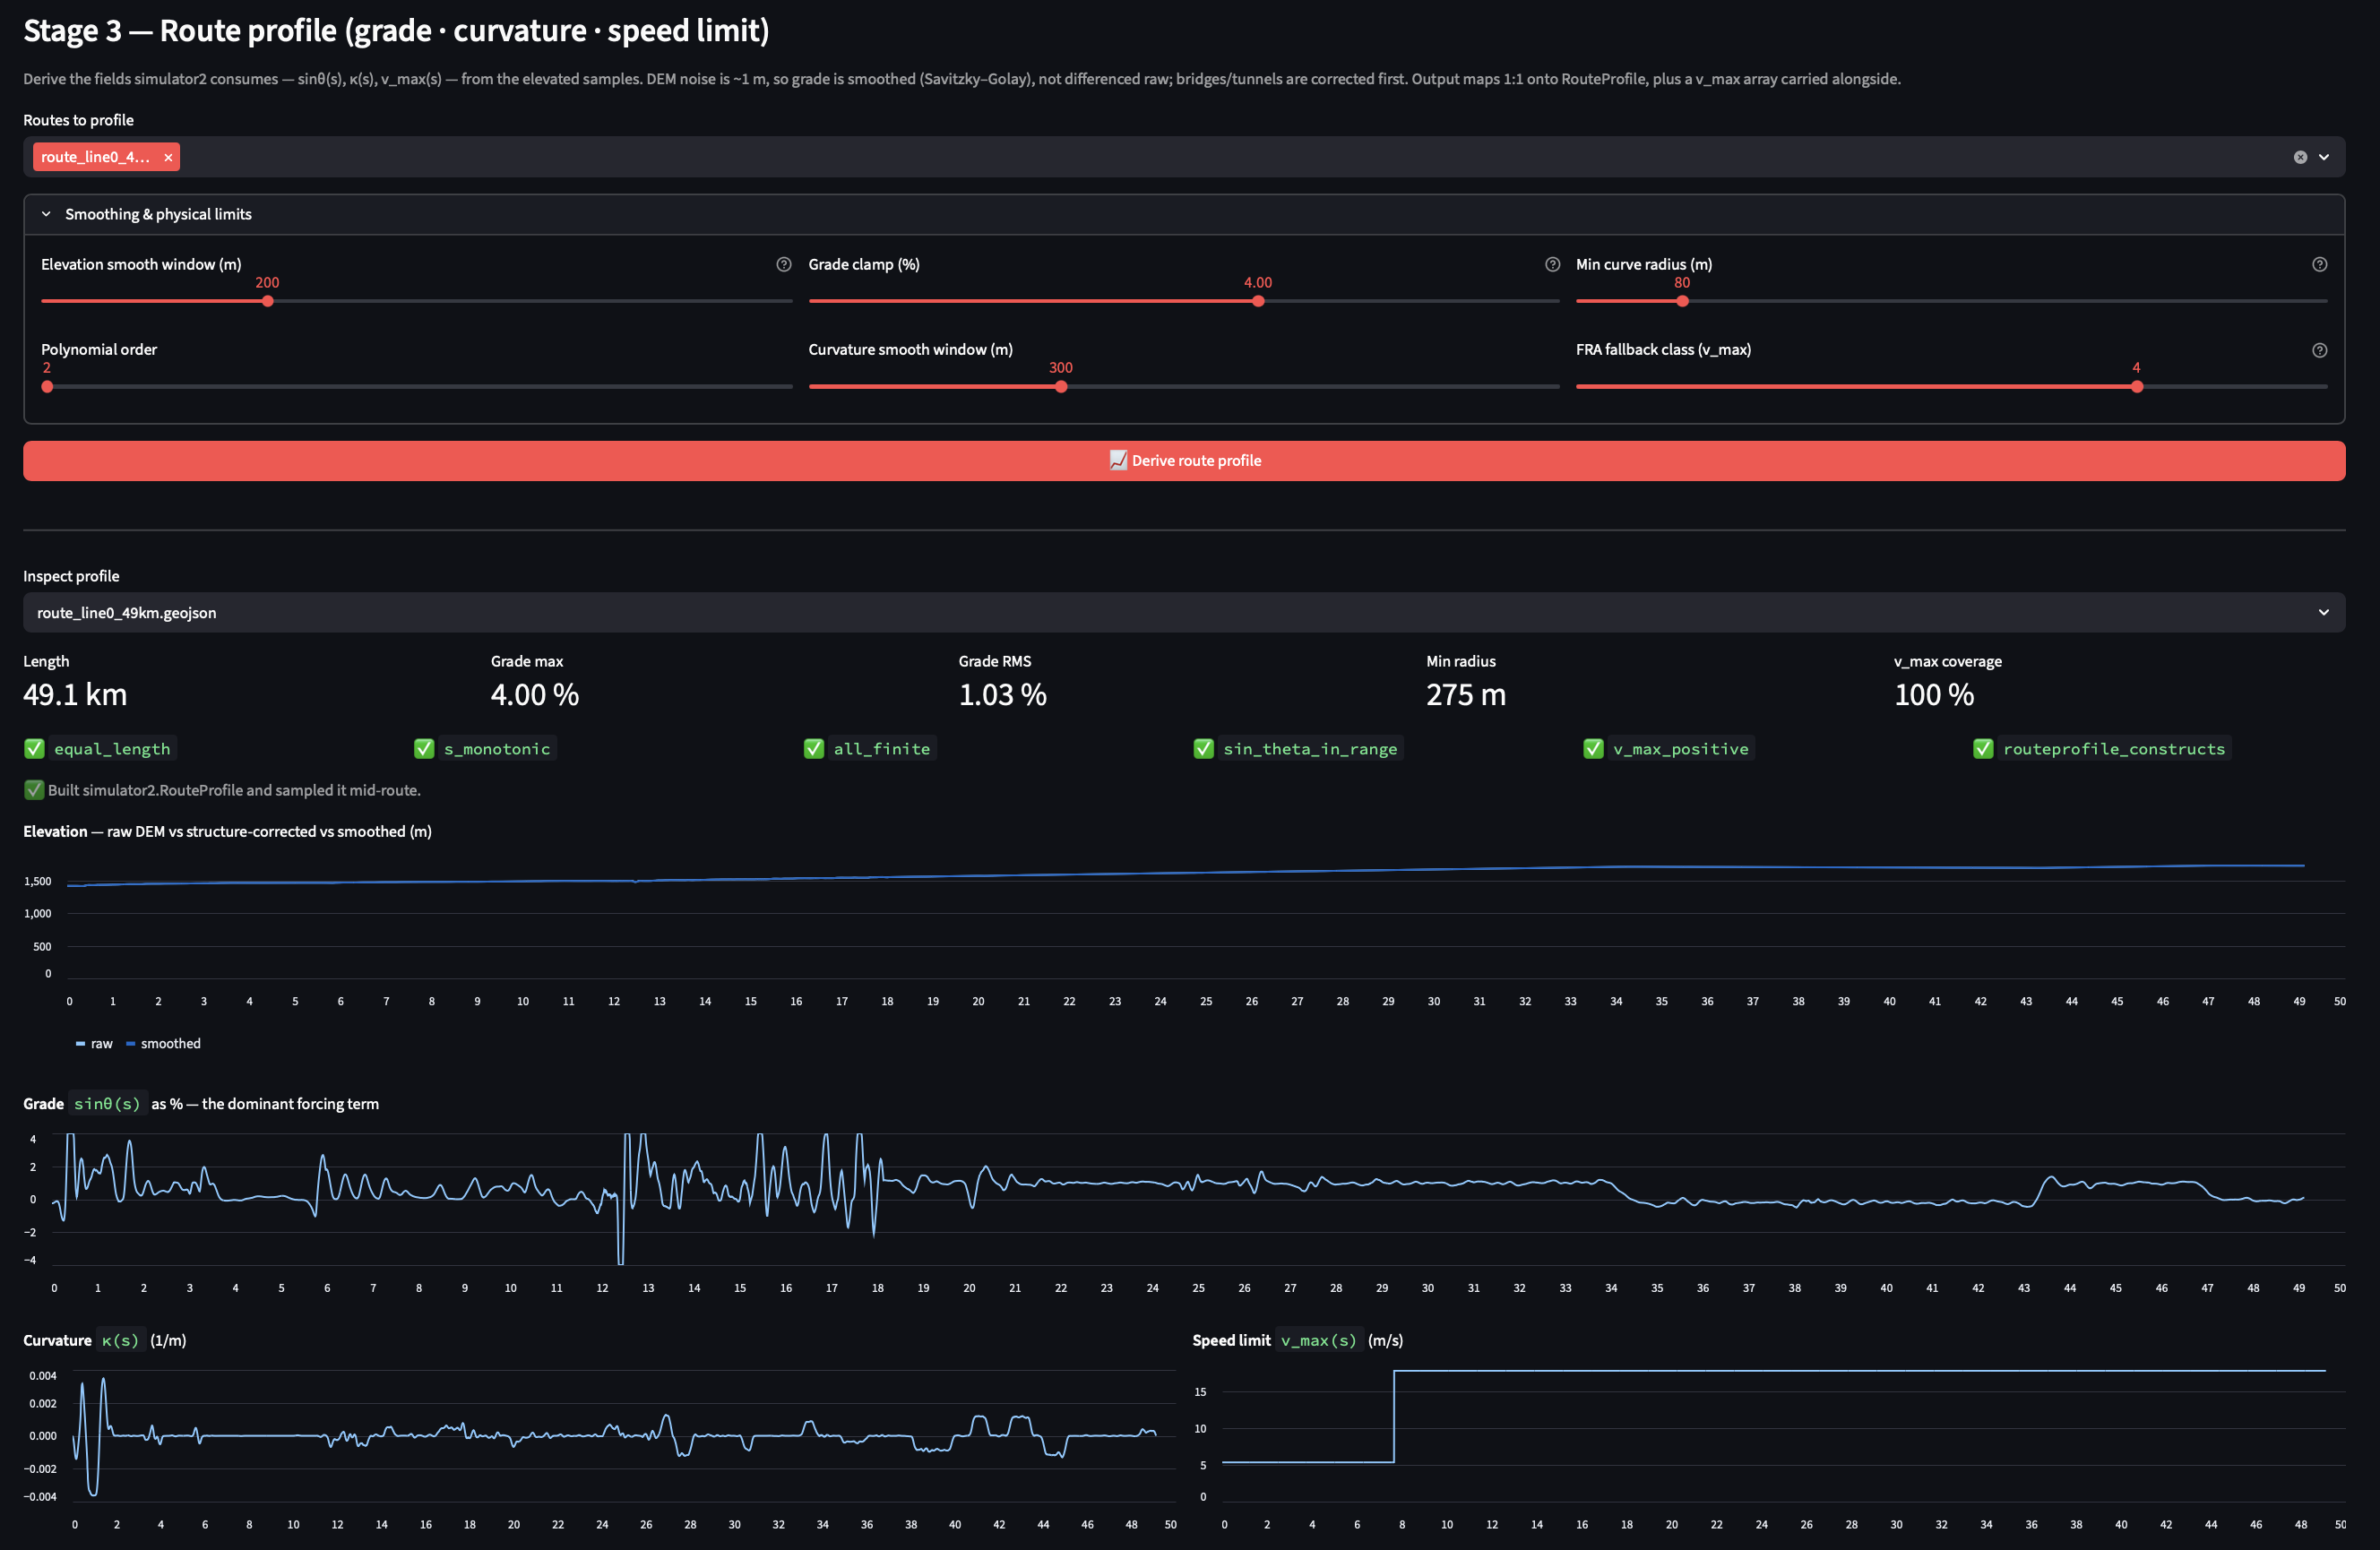
\includegraphics[width=0.82\linewidth]{figures/route_profile_app.png}}
  \caption{The route-profile stage of the acquisition console, which derives the fields the simulator consumes from the elevated samples. The controls at top set the elevation smoothing window, grade clamp, minimum curve radius, and Savitzky-Golay polynomial order; the panels below show, for the same 49~km corridor, the raw and smoothed elevation, the grade $\sin\theta(s)$ as a percentage, the curvature proxy $\kappa(s)$, and the step-valued speed limit $v_{\max}(s)$. The noisier grade over the first 20~km corresponds to the urban approach.}\label{fig:profile}
\end{figure}

\subsection{Export and Reliability}

Finished routes are collected into an export bundle: one array file per route holding exactly \texttt{route\_s}, \texttt{route\_sin\_theta}, \texttt{route\_kappa}, and \texttt{route\_vmax}; an index of each route's location, endpoints, length, and grade and curvature statistics; and a manifest recording the meaning and provenance of each channel. The array files map directly onto the simulator's route-profile input, and each is sampled through an actual route-profile object as a final check before it is trusted.

Because pulling all track in a large or dense area in a single request tends to time out, queries exclude service and industrial spurs, the seed query is split into a grid of small requests, and every request retries with exponential backoff and jitter across mirror servers. For a handful of routes the interactive application suffices; for a larger dataset, the pipeline is first verified interactively on known areas, confirming that lines render as continuous corridors, that gaps are short and located at bridges, and that traced length is plausible against an independent map. Only then is a headless batch crawler run over curated seed points, deduplicating overlapping pulls and resuming from a cache after interruption.

Two design choices run through the pipeline. First, acquisition and assembly are pure functions wherever they do not require a live network call, which makes the line-stitching logic unit-testable offline against a fixture built from a captured query response. Second, data quality problems are surfaced rather than silently patched: gaps are bridged but their size reported, and branch points flagged rather than auto-resolved, so the user decides whether a route is clean enough to use.

% ======================================================================
\section{TrainSet: A Desktop Research Console}\label{sec:trainset}
% ======================================================================

The simulator and the route pipeline are libraries, driven from notebooks and scripts, with consists, routes, and command sets assembled by hand as Python objects. This is a workable way to produce a figure but an inefficient basis for exploration, which constitutes much of the surrounding research. TrainSet is a desktop application built over the same backend. It is not a deliverable of the study in its own right, and no numerical claim depends on it; it is documented here because the way a tool shapes which questions are asked is part of the method.

\subsection{Motivation and Architecture}

Three considerations motivated its construction. The first is the cost of a question: determining what happens to coupler forces if a train is thirty cars longer on a particular grade requires, in script form, editing a consist definition, rebuilding a scenario, re-running the solver, and re-plotting, so that many such questions are never asked. The second is the gap between a number and a shape, since the failure modes that matter here, such as a run-in resolved unphysically, a grade artifact surviving the smoothing stage, or a brake command overlapping traction in a manner no operator would produce, are immediately visible in a plot yet nearly invisible in a summary statistic. The third is reproducible bookkeeping, since every object involved must be nameable, saveable, and reloadable so that a run can be repeated exactly.

The governing architectural constraint is that the user interface never imports the numerical stack. The backend packages are reached only through a thin service layer, so the backend continues to run headless: notebooks, the batch generator, and the figures in this paper have no dependency on the interface toolkit, and each service is unit-testable without a display. The boundary is also a natural insertion point, since the surrogate and controller attach as additional services without altering any existing screen. Because the simulator integrates the whole time span in one adaptive solver call, there is no intermediate hook against which to report progress or to interrupt, and the stop control is correspondingly disabled, a genuine limitation rather than an oversight, since streaming a run requires a stepwise integrator that the reference implementation deliberately does not use.

\subsection{Screens and Artifacts}

The route screen browses the output of \customref{ROUTE ACQUISITION}{sec:routes}, rendering chainage-linked elevation, grade, and curvature plots alongside a summary panel of length, elevation range, climb and descent, grade range, minimum radius, speed-limit range, and the fraction of the line for which the map actually supplied a speed limit. That last field is a data-quality property rather than a physical one, easy to overlook when a route is loaded programmatically but impossible to overlook when printed beside the grade range on every load.

The consist screen implements the three-way split around which the data model was designed: a library of reusable car types, an ordered train under construction, and a shelf of saved trains (Figure~\ref{fig:trainset}a). A car type is a named template carrying mass split into tare and lading, Davis coefficients, traction and braking ceilings, physical length, and a coupler type, stored one per file as a plain-text record so that the library is version-controllable outside the application. A train is an ordered list of references to those types, so that a train file stays small regardless of length and a correction to a car type propagates to every train that uses it. Any car may override selected fields while inheriting the rest, which makes a train with a single unusually heavy car expressible without introducing a near-duplicate type.

The consist in Figure~\ref{fig:trainset}a was produced by the procedural generator rather than assembled by hand. The generator writes through the same save path the interface uses, so generated and hand-built trains are indistinguishable downstream, which makes large training sweeps possible without a second code path. The controls screen generates driving commands. A control profile is a train-agnostic recipe, defined as piecewise command curves expressed as a fraction of each vehicle's own force ceiling rather than in newtons, so that one profile drives any consist, with knots interpolated using the same smoothstep shape as the simulator's traction ramp to avoid the stiffness that instantaneous steps introduce. Profiles are generated randomly under user-specified bounds on duration, knot count, and traction and brake fraction ranges, with a live preview of the resulting command for each power role. Distributed power units are addressed by role, namely head-end, mid-train, and rear helper, resolved from each car's label, and may be driven synchronously with a configurable lag behind the head end, independently, or not at all. Generation is seeded, so that a profile is reproducible from its configuration alone.

Randomized commands are what the surrogate's training set requires, since a model trained only on hand-designed driving would never encounter the transients that make coupler dynamics difficult, while the bounded ranges keep the randomness plausible rather than arbitrary.

The simulate screen is deliberately spare: it selects a saved train and route, sets a duration and two numerical options, selects a control profile, and runs. A run is therefore fully specified by a short list of named artifacts and four numbers, and is trivially repeatable. Results plot every vehicle's speed above every coupler's force on time-linked axes (Figure~\ref{fig:trainset}b). Plotting every vehicle rather than a summary is intentional, since the information is carried by the spread between traces, with the speed envelope widening and collapsing as slack runs in and out. That behavior is invisible in a mean, and the qualitative signature, namely oscillation that decays rather than grows and forces that remain bounded, is a check that no summary statistic provides.

\begin{figure}[!htb]
  \centering
  \fbox{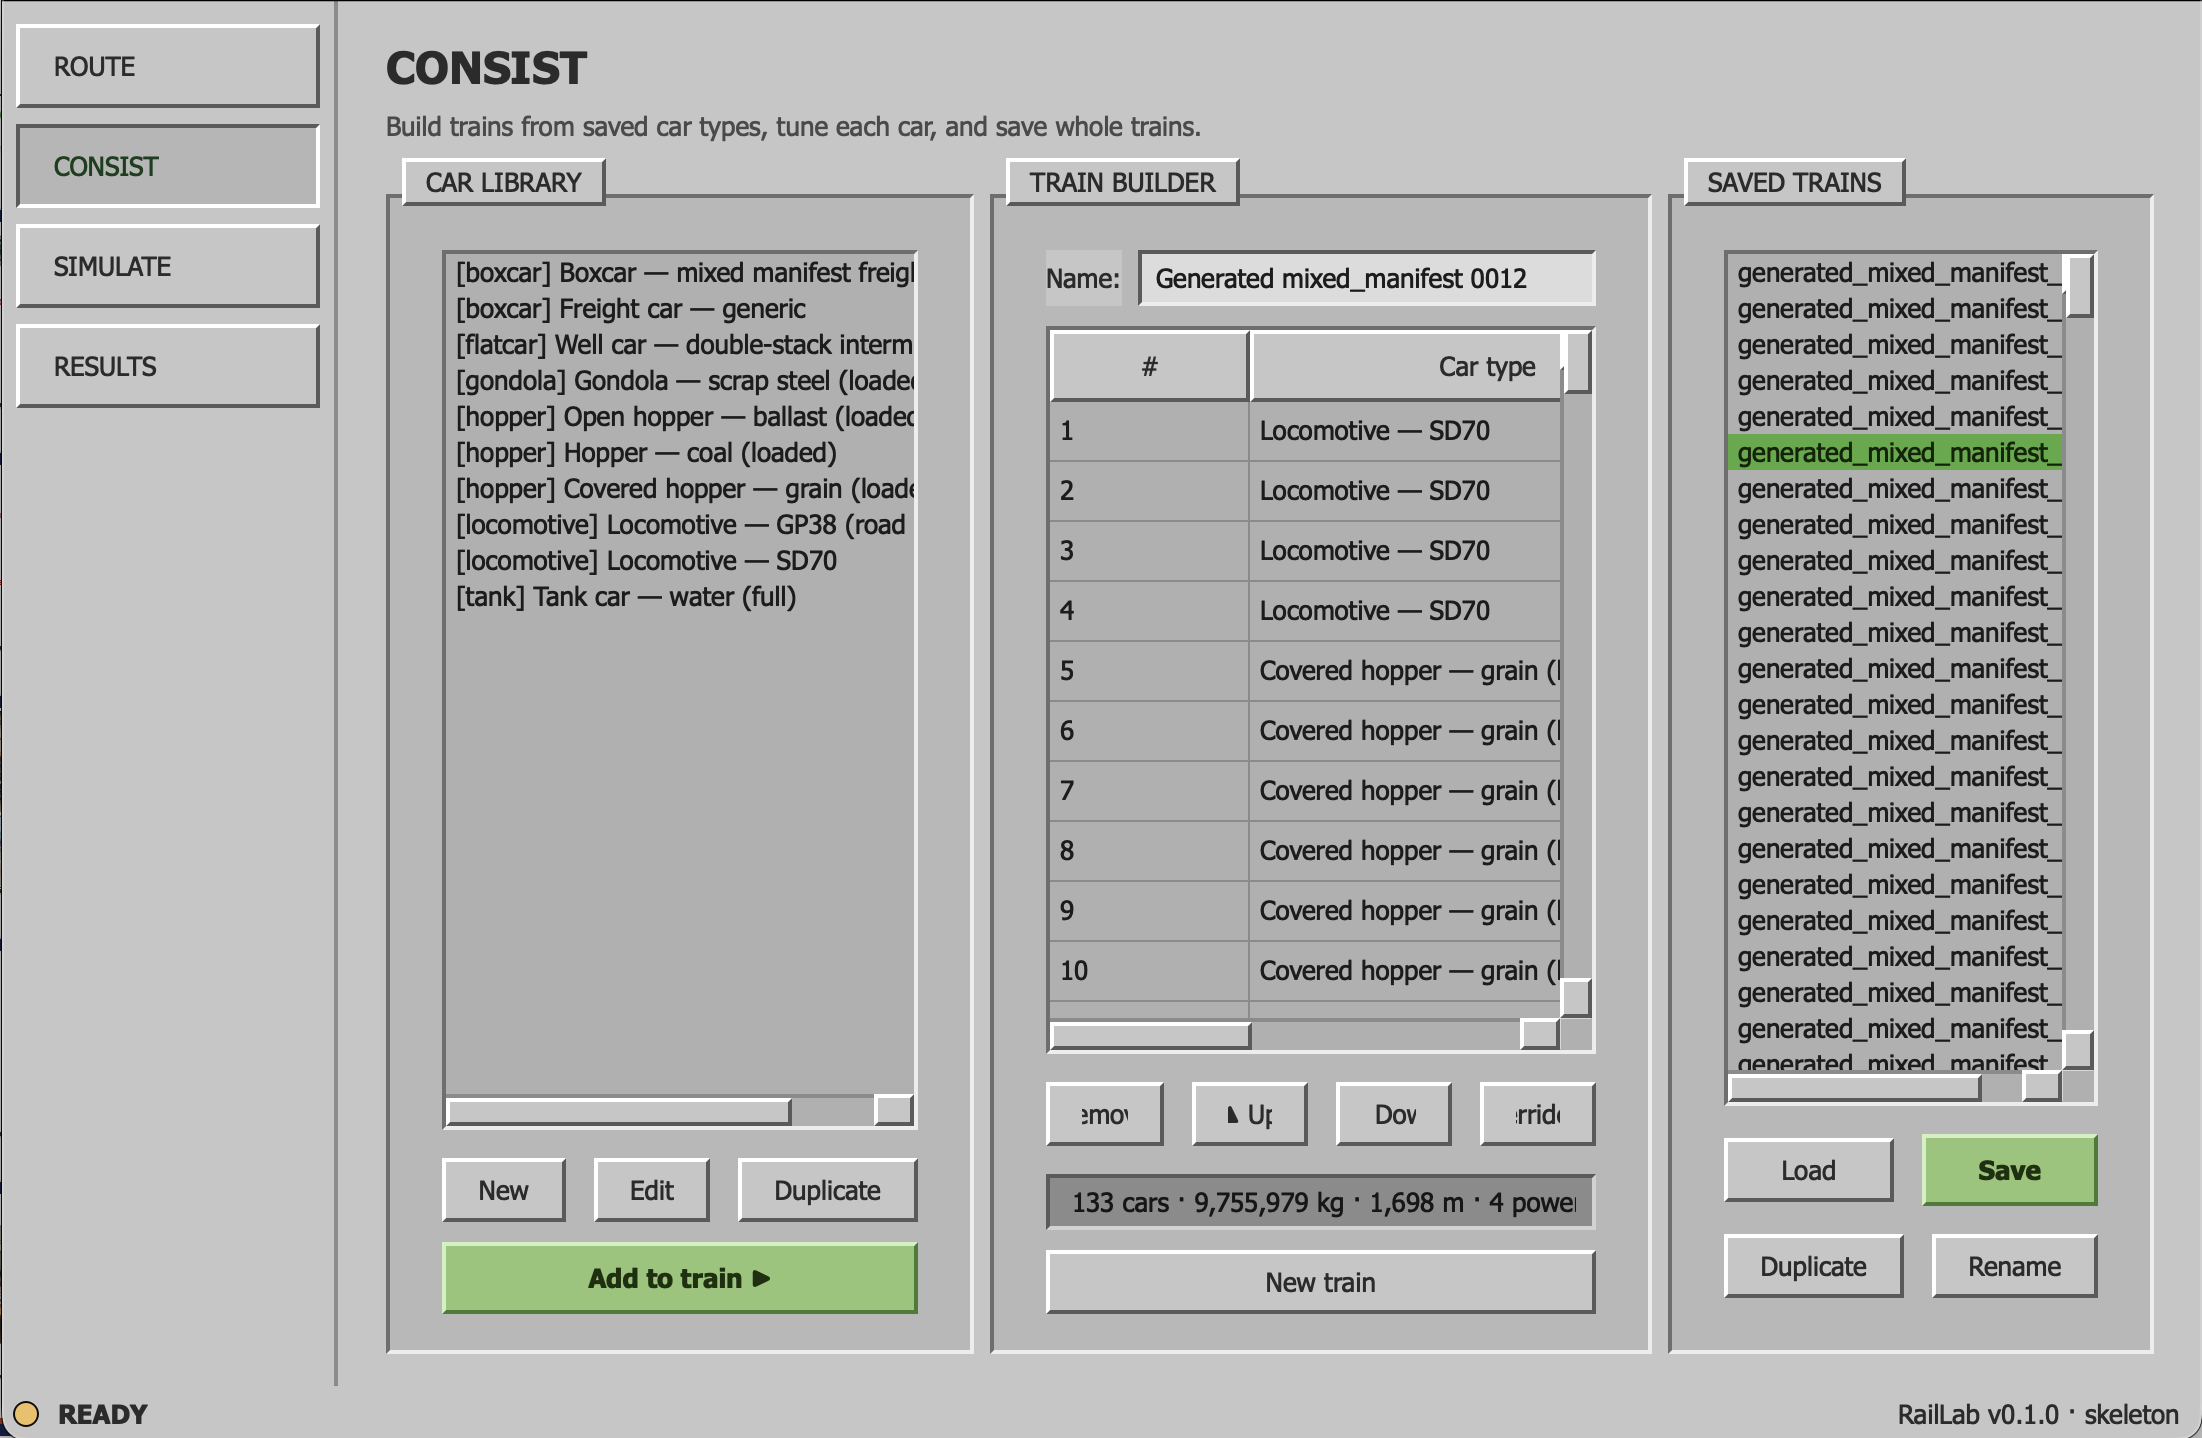
\includegraphics[width=0.55\linewidth]{figures/raillab_consist.png}}\\[2pt]
  {\footnotesize (a)}\\[6pt]
  \fbox{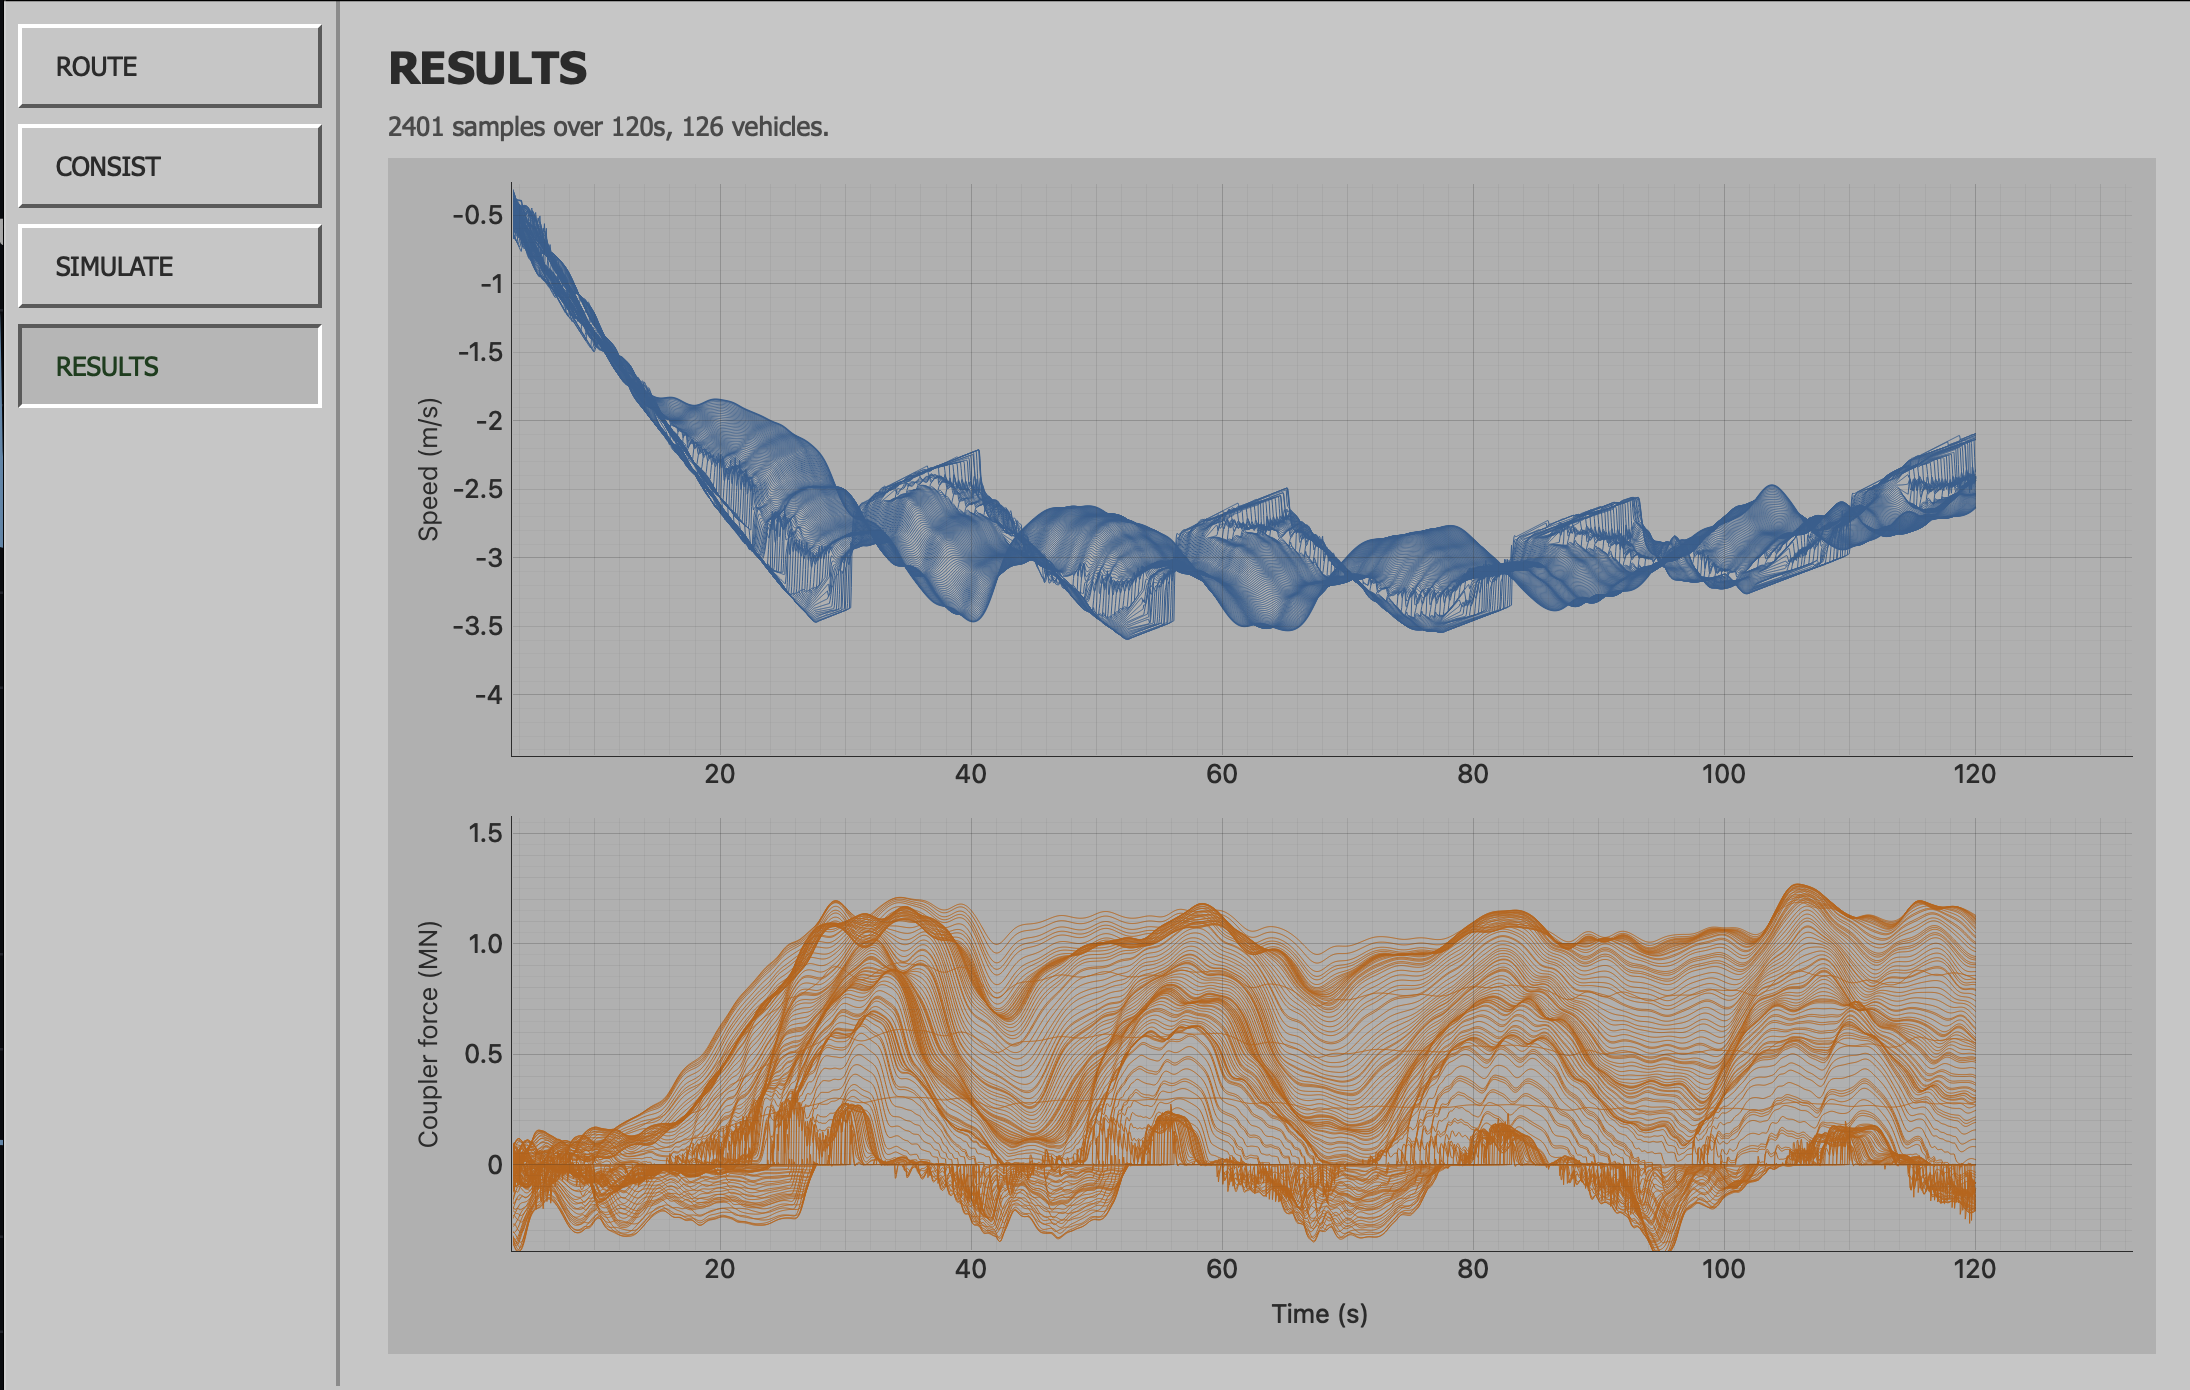
\includegraphics[width=0.55\linewidth]{figures/sim_results.png}}\\[2pt]
  {\footnotesize (b)}
  \caption{The TrainSet console. (a) The consist screen: a library of reusable car types (left), the ordered train under construction with per-car overrides (center), and saved trains (right); the train shown is a procedurally generated mixed manifest of 133 cars, roughly 9,756 tonnes and 1,698 meters long, with four powered units at the head. (b) The results screen after a 120~s run of a 126-vehicle consist under a randomized control profile: every vehicle's speed is plotted above every coupler's force on time-linked axes, and the widening and collapsing speed envelope reflects slack running in and out, with the corresponding fan of coupler forces below.}\label{fig:trainset}
\end{figure}

\subsection{Status and Limitations}

TrainSet is a working instrument rather than finished software. Runs cannot be interrupted or monitored mid-flight because the solver call is atomic, and the results screen does not yet expose the full node and edge state or export a run directly; dataset generation remains the responsibility of the headless batch path, which is the correct division of labor, since the interface is intended for examining a single run and the batch runner for producing thousands. Most importantly, nothing in the application alters the standing caveat of \customref{REFERENCE SIMULATOR}{sec:refsim}: the car-library parameters are realistic in form but are not calibrated to any specific rolling stock, and the ease of building a train and observing its behavior should not be mistaken for validation.

% ======================================================================
\section{Conclusions and Future Work}\label{sec:conclusion}
% ======================================================================

The three components compose into a single loop: a corridor is acquired from real map and elevation data and reduced to four arrays, a consist is assembled from a reusable car library, a randomized but bounded control profile is generated as a train-agnostic recipe, and the simulator integrates the result into rollout tensors in the layout of \customref{PROBLEM FORMULATION}{sec:problem}. Because the console and the batch generator share one artifact format, a run inspected interactively and a run within a million-sample training set are the same object.

This design enables the generalization experiment that the project's central claim requires. Consist length is a property of the data rather than an architectural dimension, so training on one range of lengths and evaluating on another requires no change to the model; and because routes are drawn from real corridors, whole corridors can be held out, a substantively different test from holding out synthetic variations of a single profile.

Three limitations bound what the testbed supports. First, the simulator sits at intermediate fidelity, with hysteretic draft gear, brake pipe dynamics, and adhesion limits outside its scope. Second, its parameters are illustrative rather than calibrated, so that every downstream claim concerns fidelity to this simulator rather than to real rolling stock. Third, route data quality is inherited from open sources, where DEM-derived grade is trustworthy in aggregate but degrades on urban approaches, which is why the pipeline surfaces coverage and interpolation statistics rather than smoothing them away.

Work proceeds along three lines. The immediate step is bulk dataset generation across a curated set of corridors and a randomized family of consists, with held-out corridors and consist-length ranges reserved before training begins. Next is the surrogate itself: a message-passing graph network producing the residual $\Delta\mathcal{F}_\theta$ of Equation~\ref{eq:node_evolution}, integrated as a neural ODE and trained against Equation~\ref{eq:loss}, and benchmarked against physics-only and physics-residual multilayer-perceptron baselines as well as a transformer variant that tests whether the graph structure earns its place. Finally, the trained surrogate becomes the differentiable world model within a model-predictive control routine minimizing trip energy on held-out routes subject to speed limits and coupler-force constraints.

No surrogate is trained in this paper, and no accuracy or speedup is claimed. What is established is that the phenomena distinguishing LTD from point-mass modeling are reproduced on corridors derived from real track, at consist sizes above 120 vehicles, under randomized driving commands, and in a form that can be generated in bulk and held out by corridor, the precondition for the modeling and control results to follow.

% ======================================================================
\section{Acknowledgments}
% ======================================================================

The authors thank the School of Engineering at Colorado State University Pueblo. Route geometry is derived from OpenStreetMap, \textcopyright{} OpenStreetMap contributors, available under the Open Database License; elevation data are from the U.S. Geological Survey 3D Elevation Program. This work was supported by the Federal Railroad Administration's Consolidated Rail Infrastructure and Safety Improvements (CRISI) Program through a railway workforce development project led by the Center for Urban Transportation Research at the University of South Florida.

% ---------- Author Contributions ----------
% TODO: verify CRediT role assignment before submission.
\section*{AUTHOR CONTRIBUTIONS}
The authors confirm their contributions to the paper as follows. George James: conceptualization, methodology, software, data curation, formal analysis, visualization, and writing of the original draft. Trung Duong: conceptualization, methodology, supervision, validation, and review and editing. Md Islam: funding acquisition, project administration, resources, supervision, and review and editing. Saqib Gulzar: project administration, supervision, and review and editing. All authors reviewed and approved the final manuscript.

% ---------- Declaration of COI ----------
% TODO: confirm before submission.
\section*{DECLARATION OF CONFLICTING INTERESTS}
The authors declared no potential conflicts of interest with respect to the research, authorship, or publication of this article.

\bibliographystyle{trb}
\bibliography{ltd_surrogate_trb}

\end{document}
